%Thanks to Prof. Bazioch for the use of his template
%TeXMaker on a PC or Linux and TeXShop on a mac are good editors for
%creating LaTeX documents
%A good place to get started with LaTeX is
%http://ctan.mirrors.hoobly.com/info/Math_into_LaTeX-4/Short_Course.pdf
\documentclass[12pt]{article}
\usepackage{amsmath,amssymb,amsthm}
\usepackage{graphicx}
\usepackage{xfrac}
\usepackage{caption}
\usepackage{subcaption}
\usepackage{enumerate,multicol,verbatim}
\usepackage{fullpage}

\setlength{\parindent}{0in}
\setlength{\parskip}{3mm}
\newcommand{\nline}{\rule{\linewidth}{0.5pt}}

\theoremstyle{plain}
\newtheorem{theorem}{Theorem}
\newtheorem{lemma}[theorem]{Lemma}
\newtheorem{proposition}[theorem]{Proposition}
\newtheorem{corollary}[theorem]{Corollary}

\theoremstyle{definition}
\newtheorem{definition}[theorem]{Definition}
\newtheorem{notation}[theorem]{Notation}
\newtheorem{remark}[theorem]{Remark}
\newtheorem{note}[theorem]{Note}
\newtheorem{nn}[theorem]{}



% document title YOU DO NOT NEED TO CHANGE THIS
\makeatletter
\renewcommand{\maketitle}{
\begin{center}
\nline\\
\vspace{2ex}
{\huge \textsc{\@title}}
\nline\\
{\large\textsc{\@author \hfill \@date}}
\vspace{4ex}
\end{center}
}
\makeatother
%%%

%%%%%%%%%%%%%%%%%%%%%%%%%%%%%%%
%%%%%%%%%%%%%%%%%%%%%%%%%%%%%%%

%%%%%%% THIS SHOULD BE CHANGED FOR EACH NEW ASSIGNMENT

\title{HPC I Homework 3}

%%%%%%% BE SURE TO PUT IN YOUR OWN NAME

\author{Morse, Michael}

%%%%%%% BE SURE TO PUT IN THE DUE DATE

\date{December 11, 2017}

%%%%%%%%%%%%%%%%%%%%%%%%%%%%%%%
%%%%%%%%%%%%%%%%%%%%%%%%%%%%%%%


\begin{document}

\maketitle
\newpage
%%%%%%%%%%%%%%%%%%%%%%%%%%%%%%%
%Problem 1
%%%%%%%%%%%%%%%%%%%%%%%%%%%%%%%

\section{Problem 1}
\subsection{Strong Scaling}
\begin{figure*}[t]
    \centering
    \begin{subfigure}[t]{0.5\textwidth}
        \centering
        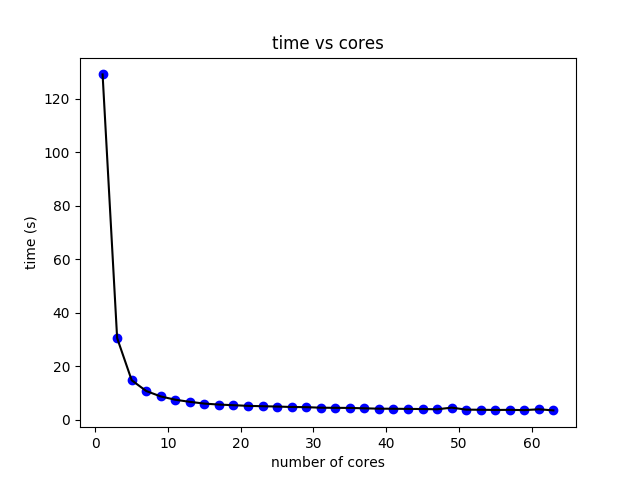
\includegraphics[height=2.2in]{timeq1_strong.png}
         \caption{Time vs number of cores}
    \end{subfigure}%
    ~
    \begin{subfigure}[t]{0.5\textwidth}
        \centering
        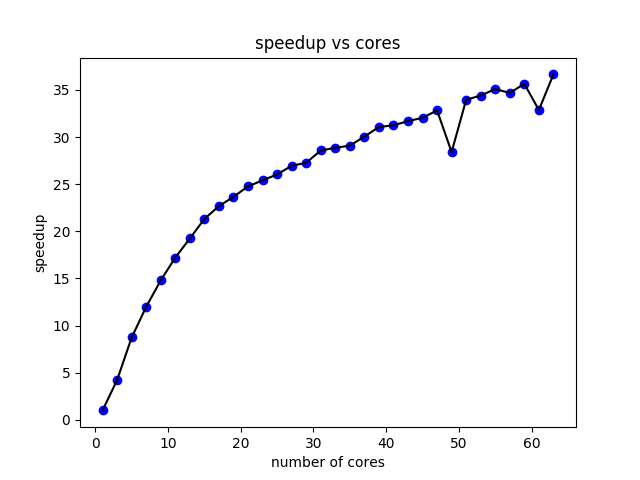
\includegraphics[height=2.2in]{speedupq1_strong.png}
        \caption{Speed-up vs number of cores}
    \end{subfigure}
    \caption{Plots for Round Robin Mandelbrot code}
    \label{fig:q1a}
\end{figure*}

For my round robin Mandelbrot code I used two processors as the serial time $T_1$ as one processor was the master so only one was doing the work. The code was has nearly linear speedup up to around 20 cores then again after around 25 cores. I believe that this is around the time that communication between nodes comes into play. Unfortuntely, attempting to use the beginning point to estimate the serial fraction of the code by 
\begin{equation}
S = (1-F_s)p + F_s
\end{equation} 
was unsuccessful as $F_s$ was given as $F_s \approx -0.7$ from both the slope and the y-intercept. This leads me to believe that the communication time is non-negligible. However, we can use Eqn.(9) from chapter 2 of Eijhout's book, and some algebra to write
\begin{equation}
\frac{1}{S} = F_p (\frac{1}{p}) + (1-F_p)
\end{equation}  
where we have assumed that the communication time is a constant. Using scipy statistics we get that the code has a $F_p = .95$ with a $r^2 = .97$. We should expect that is code is almost perfectly parallelizable as the only parts done in serial are the check on the point and the initialization, both of which are not mathematically intensive. This can be seen in Fig.(\ref{fig:inverse1a}).
\begin{figure}
        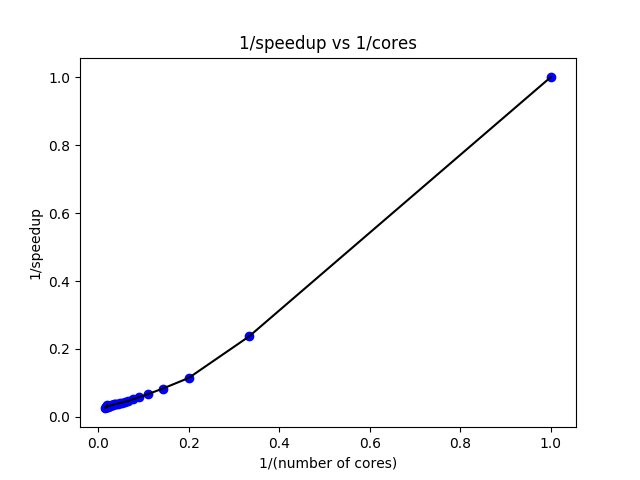
\includegraphics[width=0.5\textwidth]{inverseq1_strong.png}
        \caption{$\sfrac{1}{\mathrm{Speed-up}}$ vs $\sfrac{1}{\mathrm{number of cores}}$}
        \label{fig:inverse1a}
\end{figure}

 
\subsection{Karp-Flatt metric}
We can use also calculate the serial fraction using the Karp-Flatt metric defined as 
\begin{equation}
f_s = \frac{\frac{1}{s}-\frac{1}{p}}{1-\frac{1}{p}}
\end{equation}
Taking the average of the $f_s$ calculated for 2-36 cores we get that for the Mandelbrot set code $f_s = 0.02 \pm 0.17$ which is consistent with the $f_s$ calculated in the first subsection of $0.05$

\subsection{Weak Scaling}



\section{Problem 2}
\subsection{Strong Scaling}
\begin{figure*}[t]
    \centering
    \begin{subfigure}[t]{0.5\textwidth}
        \centering
        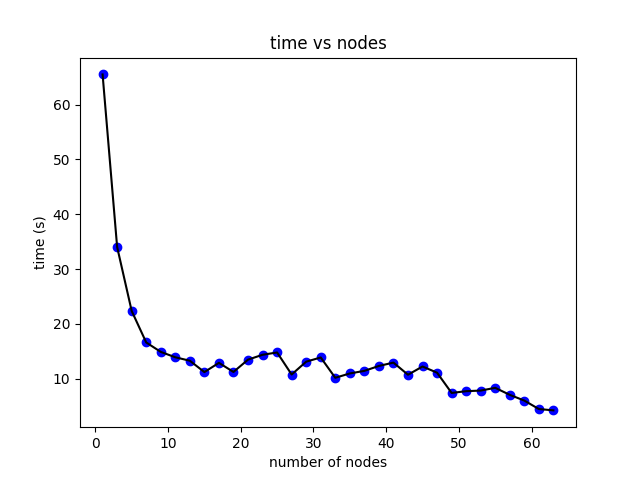
\includegraphics[height=2.2in]{timeq2_strong.png}
         \caption{Time vs number of cores}
    \end{subfigure}%
    ~
    \begin{subfigure}[t]{0.5\textwidth}
        \centering
        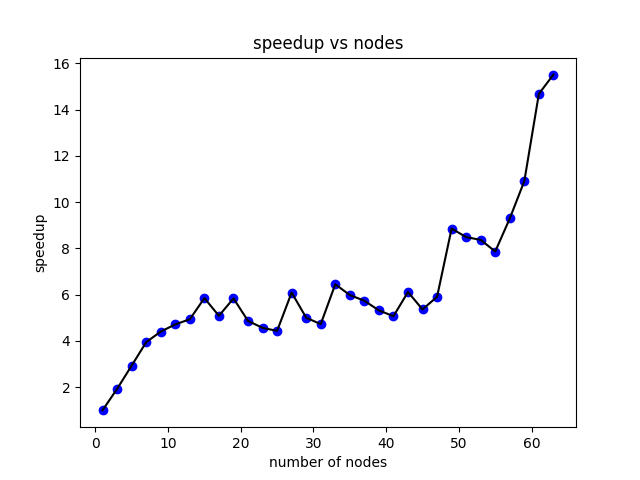
\includegraphics[height=2.2in]{speedupq2_strong.png}
        \caption{Speed-up vs number of cores}
    \end{subfigure}
    \caption{Plots for pi code}
    \label{fig:q2a}
\end{figure*}

We can run the same type of analysis we did in question 1 on the pi code used as an example in \textit{Using MPI} by Gropp. We notice first in Fig.(\ref{fig:q2a}) that the speed-up and time decrease lines are not as sharp as they are in question 1. I would postulate that this is because there is more work being done serially and as there is 

\begin{figure}
        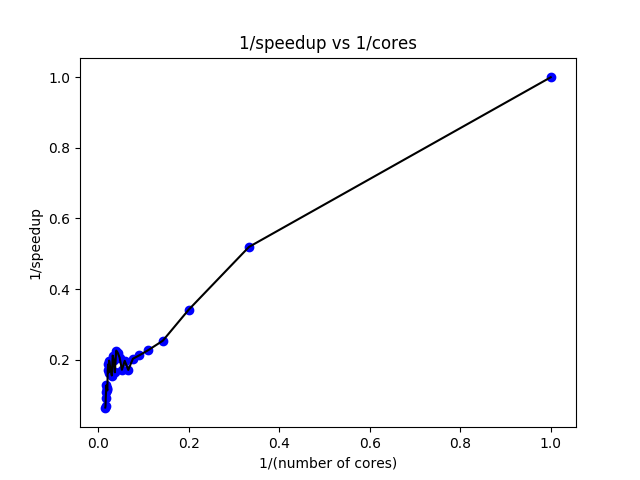
\includegraphics[width=0.5\textwidth]{inverseq2_strong.png}
        \caption{$\sfrac{1}{\mathrm{Speed-up}}$ vs $\sfrac{1}{\mathrm{number of cores}}$}
        \label{fig:inverse1a}
\end{figure}


%\begin{figure}
%\label{fig:problem3}
%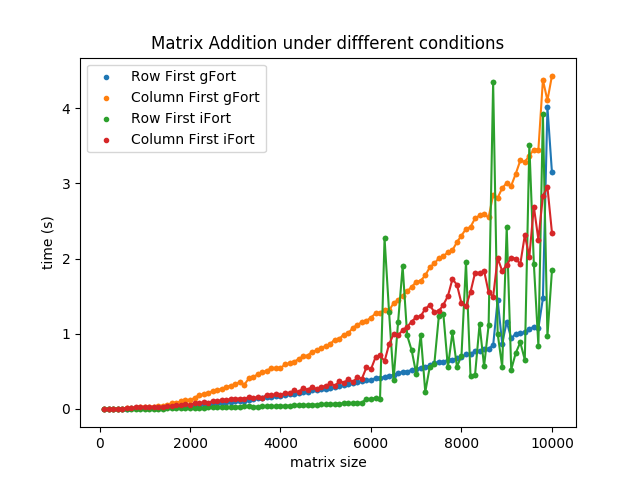
\includegraphics[scale=0.7]{problem3.png}
%\caption{Matrix addition with different compilers and ordering}
%\end{figure}

\end{document}